\documentclass{article}
\usepackage[utf8]{inputenc}
\usepackage[ukrainian]{babel}
\usepackage{graphicx}
\usepackage{hyperref}
\usepackage{tabularx}
\usepackage{booktabs}
\usepackage{xcolor}
\usepackage{subcaption}
\usepackage{float}

\title{Модель пухлини на основі клітинного автомата}
\date{}

\begin{document}

\maketitle

\tableofcontents

\newpage

\section{Вступ}
Ракові захворювання є досить великою проблемо в сучасному світі, і нажаль ця проблема лише набирає обертів. Для кращого вивчення розвитку раку існують математичні моделі. Цей проєкт є однією з них, а точніше це симуляція що базується на клітинному автоматі.

\section{Теоретичні основи}
\subsection{Клітинні автомати в моделюванні раку}
Клітинний автомат базується на дискретному полі NxN, що при досить великиз значеннях надає досить точні та реалістичні результати. Клітинні автомати використовують стокастичний метод ітерування, тобто на кожному кроці дію клітини визначає якась випадкова подія. На клітину може впливати її оточення, наприклад концентрація ракових клітин. В цій симуляції на клітину впливають лише 8 сусідів розташованих у квадраті 3х3 з центром у даній.

\subsection{Ієрархія клітин пухлини}
Типи клітин використаних у симуляції:
\begin{itemize}
    \item Істинні стовбурові клітини (TSC) - клітини що не вмирають, можуть народжувати як собі подібних, так і і звичайні стовбурові клітини.
    \item Стовбурові пухлинні клітини (STC) - можуть лише звичайні ракові пухлини
    \item Звичайні пухлинні клітини (RTC) - пухлини, що породжують собіподібних, проте мають обмежену кількість поділів.
    \item Некротичні клітини - мертві клітини.
    \item Імунні клітини - клітини, що вюивають рак або вповільнюють його поділ.
\end{itemize}

\subsection{Динаміка росту пухлини}
Основні події життєвого циклу клітин:
\begin{itemize}
    \item Поділ
    \item Міграція
    \item Смерть
    \item Вибір шляху диференціації
\end{itemize}

\subsection{Взаємодія з імунною системою}
Механізми імунної відповіді:
\begin{itemize}
    \item Активація
    \item Знищення клітин пухлини
    \item Міграція та поділ імунних клітин
    \item Тривалість життя імунних клітин
\end{itemize}

\section{Реалізація}
\subsection{Архітектура моделі}
\begin{itemize}
    \item Решітка (Grid)
    \item Клас клітин (Cell)
    \item Симулятор (TumorSimulation)
\end{itemize}

\subsection{Основні параметри}

У цьому розділі коротко описуються ключові параметри, що використовуються в моделі.

\subsection{Алгоритм симуляції}
Покроковий опис:
\begin{enumerate}
    \item Оновлення клітин пухлини
    \item Оновлення імунних клітин (якщо увімкнено)
    \item Збір статистики
\end{enumerate}

\section{Результати симуляції}

\subsection{Візуалізація та колірна схема}

Для інтерпретації результатів симуляції застосовується наступна колірна схема клітин:

\begin{itemize}
    \item \textcolor{blue}{\rule{1em}{1em}} Імунні клітини (Immune cells)
    \item \textcolor{orange}{\rule{1em}{1em}} Некротичні клітини (Necrotic cells)
    \item \textcolor{gray}{\rule{1em}{1em}} Порожні клітини (вільний простір)
    \item \textcolor{yellow}{\rule{1em}{1em}} Істинні стовбурові клітини (True Stem Cells)
    \item \textcolor{green}{\rule{1em}{1em}} Стовбурові пухлинні клітини (Stem Tumor Cells)
    \item \textcolor{red}{\rule{1em}{1em}} Звичайні пухлинні клітини (Regular Tumor Cells), з градацією відтінків залежно від кількості поділів
\end{itemize}

\subsection{Динаміка росту пухлини без імунної відповіді}
На рисунках нижче показано просторову динаміку росту пухлини без впливу імунної системи. Видно поступове збільшення маси пухлини та утворення некротичного ядра.

\begin{figure}[H]
    \centering
    \begin{subfigure}[t]{0.32\linewidth}
        \centering
        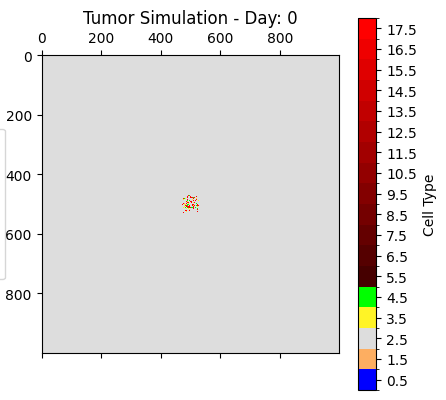
\includegraphics[width=\linewidth]{tumor_simulation_stats/tumor_day_0.png}
        \caption{День 0}
        \label{fig:tumor-day-0-no-immune}
    \end{subfigure}
    \hfill
    \begin{subfigure}[t]{0.32\linewidth}
        \centering
        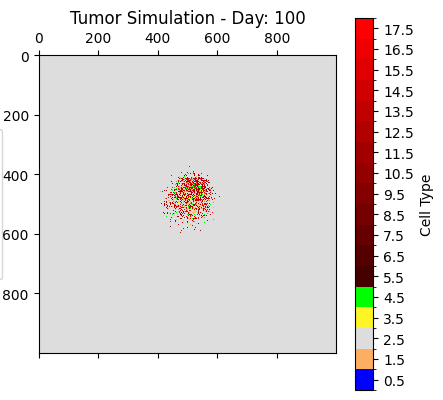
\includegraphics[width=\linewidth]{tumor_simulation_stats/tumor_day_100.png}
        \caption{День 100}
        \label{fig:tumor-day-100-no-immune}
    \end{subfigure}
    \hfill
    \begin{subfigure}[t]{0.32\linewidth}
        \centering
        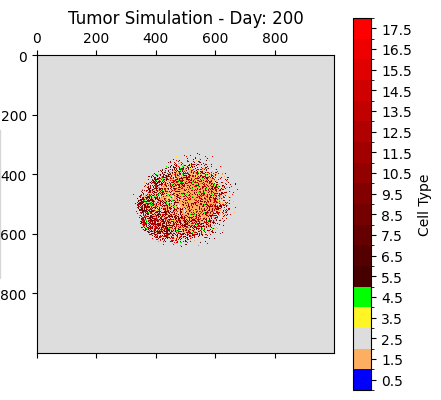
\includegraphics[width=\linewidth]{tumor_simulation_stats/tumor_day_200.png}
        \caption{День 200}
        \label{fig:tumor-day-200-no-immune}
    \end{subfigure}
    \label{fig:tumor-evolution-no-immune}
\end{figure}

\subsection{Динаміка росту пухлини з імунною відповіддю}
Далі представлено вплив імунної системи на динаміку пухлини. Імунні клітини поступово проникають у пухлину, взаємодіють з нею, зменшуючи кількість активних пухлинних клітин.

\begin{figure}[H]
    \centering
    \begin{subfigure}[t]{0.32\linewidth}
        \centering
        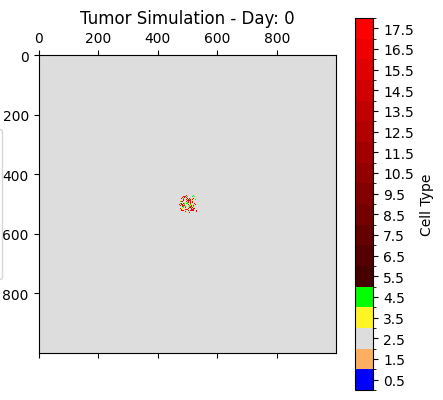
\includegraphics[width=\linewidth]{tumor_immune_simulation_stats/tumor_immune_day_0.png}
        \caption{День 0}
        \label{fig:tumor-day-0-immune}
    \end{subfigure}
    \hfill
    \begin{subfigure}[t]{0.32\linewidth}
        \centering
        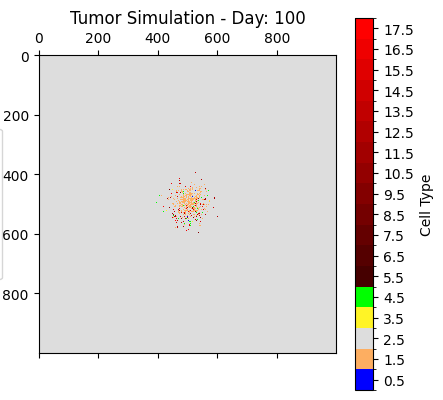
\includegraphics[width=\linewidth]{tumor_immune_simulation_stats/tumor_immune_day_100.png}
        \caption{День 100}
        \label{fig:tumor-day-100-immune}
    \end{subfigure}
    \hfill
    \begin{subfigure}[t]{0.32\linewidth}
        \centering
        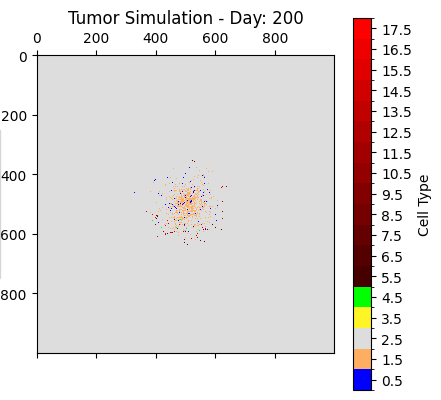
\includegraphics[width=\linewidth]{tumor_immune_simulation_stats/tumor_immune_day_200.png}
        \caption{День 200}
        \label{fig:tumor-day-200-immune}
    \end{subfigure}
    \label{fig:tumor-evolution-immune}
\end{figure}

\subsection{Графіки популяцій клітин}
На графіках показано кількісні зміни популяцій клітин протягом симуляції. Це дозволяє оцінити темпи росту пухлини, активність імунної системи, а також частку некротичних клітин.

\begin{figure}[H]
    \centering
    \begin{subfigure}[t]{0.75\linewidth}
        \centering
        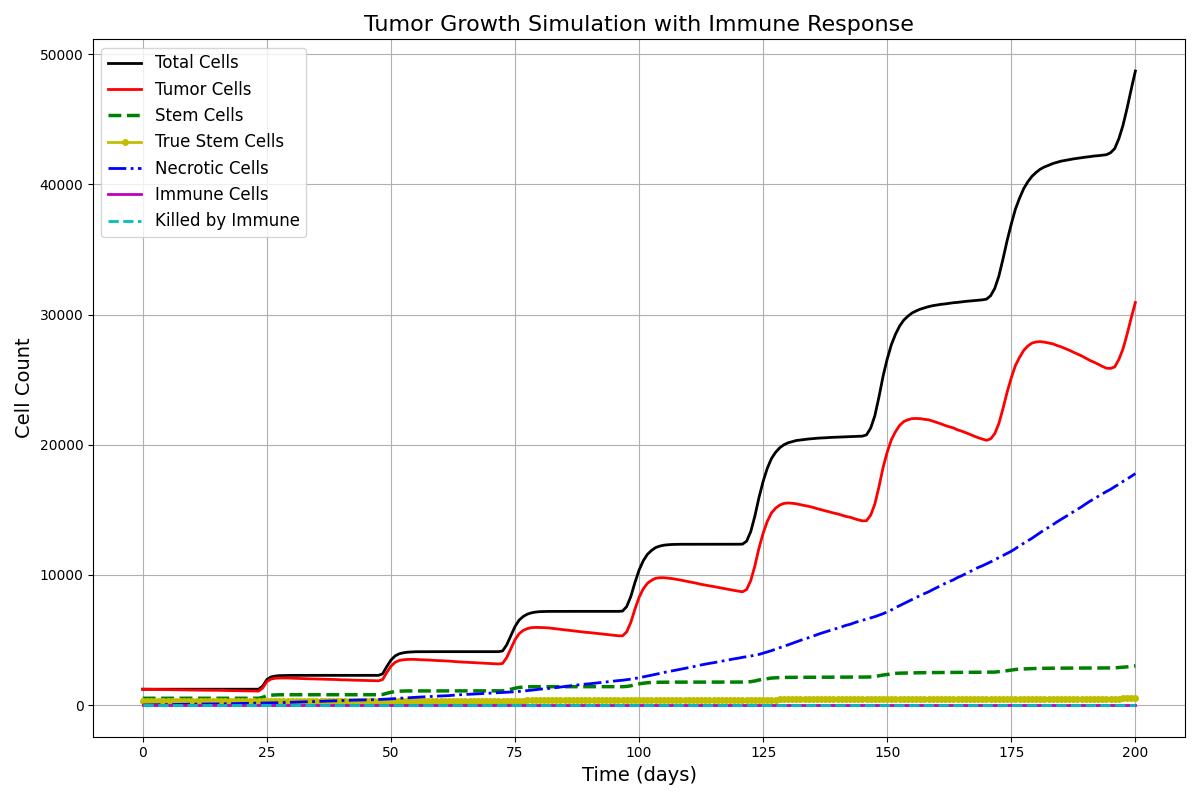
\includegraphics[width=\linewidth]{tumor_simulation_stats/tumor_stats.png}
        \caption{Динаміка популяцій клітин без імунної відповіді}
        \label{fig:tumor-stats-no-immune}
    \end{subfigure}
    
    \begin{subfigure}[t]{0.75\linewidth}
        \centering
        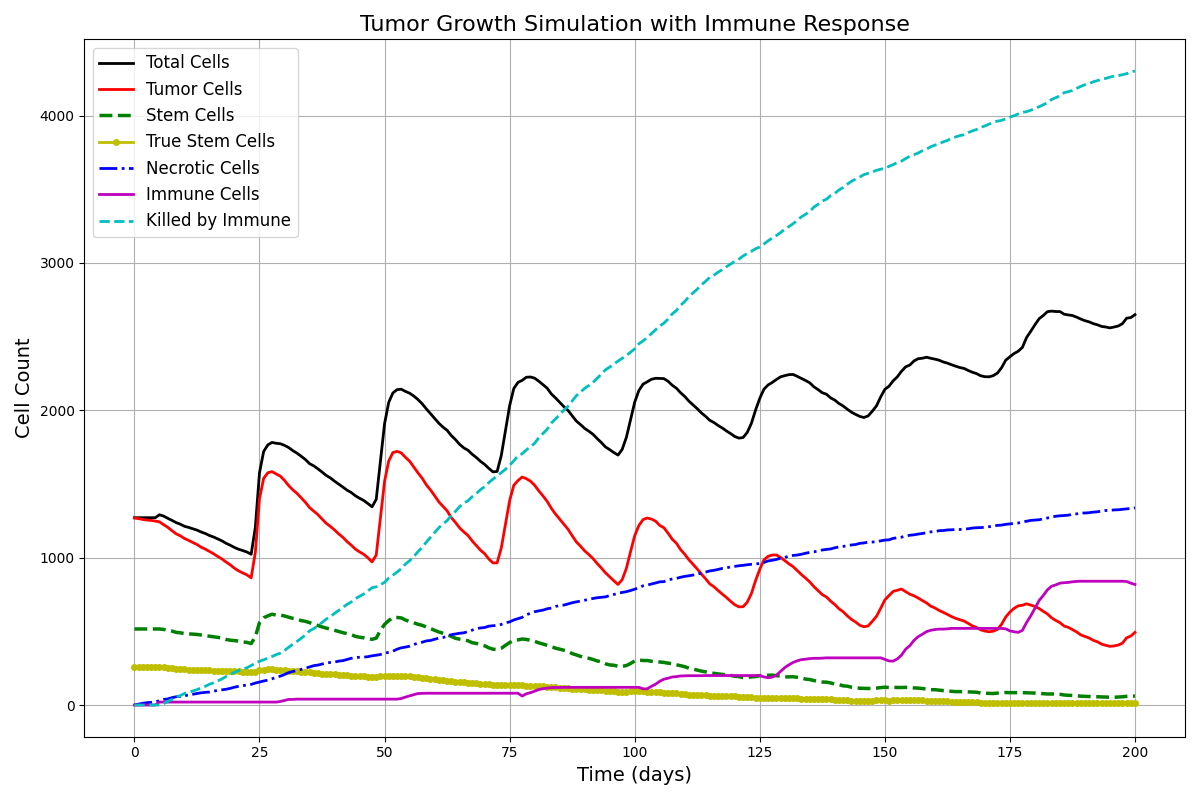
\includegraphics[width=\linewidth]{tumor_immune_simulation_stats/tumor_immune_stats.png}
        \caption{Динаміка популяцій клітин з імунною відповіддю}
        \label{fig:tumor-stats-immune}
    \end{subfigure}
    \label{fig:stats-comparison}
\end{figure}

\section{Учасники проєкту}
\begin{itemize}
    \item Ярина Печененко – логіка клітин
    \item Іван Зарицький – візуалізація, CLI
    \item Михайло Рихальський – структура решітки, просторова логіка
    \item Роман Прохоров – движок симуляції
\end{itemize}

\section{Ментор}
Максим Жук

\end{document}